\documentclass[12pt]{report}
\usepackage[utf8]{inputenc}
\usepackage[russian]{babel}
%\usepackage[14pt]{extsizes}
\usepackage{listings}
\usepackage{graphicx}
\usepackage{amsmath,amsfonts,amssymb,amsthm,mathtools} 
\usepackage{pgfplots}
\usepackage{filecontents}
\usepackage{indentfirst}
\usepackage{eucal}
\usepackage{enumitem}
\frenchspacing

\usepackage{indentfirst} % Красная строка


\usetikzlibrary{datavisualization}
\usetikzlibrary{datavisualization.formats.functions}

\usepackage{amsmath}




% Для листинга кода:
\lstset{ %
language=python,                 % выбор языка для подсветки
basicstyle=\small\sffamily, % размер и начертание шрифта для подсветки кода
numbers=left,               % где поставить нумерацию строк (слева\справа)
numberstyle=\tiny,           % размер шрифта для номеров строк
stepnumber=1,                   % размер шага между двумя номерами строк
numbersep=5pt,                % как далеко отстоят номера строк от подсвечиваемого кода
showspaces=false,            % показывать или нет пробелы специальными отступами
showstringspaces=false,      % показывать или нет пробелы в строках
showtabs=false,             % показывать или нет табуляцию в строках
frame=single,              % рисовать рамку вокруг кода
tabsize=2,                 % размер табуляции по умолчанию равен 2 пробелам
captionpos=t,              % позиция заголовка вверху [t] или внизу [b] 
breaklines=true,           % автоматически переносить строки (да\нет)
breakatwhitespace=false, % переносить строки только если есть пробел
escapeinside={\#*}{*)}   % если нужно добавить комментарии в коде
}

\usepackage[left=2cm,right=2cm, top=2cm,bottom=2cm,bindingoffset=0cm]{geometry}
% Для измененных титулов глав:
\usepackage{titlesec, blindtext, color} % подключаем нужные пакеты
\definecolor{gray75}{gray}{0.75} % определяем цвет
\newcommand{\hsp}{\hspace{20pt}} % длина линии в 20pt
% titleformat определяет стиль
\titleformat{\chapter}[hang]{\Huge\bfseries}{\thechapter\hsp\textcolor{gray75}{|}\hsp}{0pt}{\Huge\bfseries}


% plot
\usepackage{pgfplots}
\usepackage{filecontents}
\usetikzlibrary{datavisualization}
\usetikzlibrary{datavisualization.formats.functions}

\begin{document}
\thispagestyle{empty}
\begin{titlepage}
	\noindent \begin{minipage}{0.15\textwidth}
	
\includegraphics[width=\linewidth]{b_logo}
	\end{minipage}
	\noindent\begin{minipage}{0.9\textwidth}\centering
		\textbf{Министерство науки и высшего образования Российской Федерации}\\
		\textbf{Федеральное государственное бюджетное образовательное учреждение высшего образования}\\
		\textbf{~~~«Московский государственный технический университет имени Н.Э.~Баумана}\\
		\textbf{(национальный исследовательский университет)»}\\
		\textbf{(МГТУ им. Н.Э.~Баумана)}
	\end{minipage}
	
	\noindent\rule{18cm}{3pt}
	\newline\newline
	\noindent ФАКУЛЬТЕТ $\underline{\text{«Информатика и системы управления»}}$ \newline\newline
	\noindent КАФЕДРА $\underline{\text{«Программное обеспечение ЭВМ и информационные технологии»}}$\newline\newline\newline\newline\newline
	
	
	\begin{center}
		\noindent\begin{minipage}{1.3\textwidth}\centering
			\Large\textbf{  Отчет по лабораторной работе №3}\newline
			\textbf{по дисциплине "Анализ алгоритмов"}\newline\newline
		\end{minipage}
	\end{center}
	
	\noindent\textbf{Тема} $\underline{\text{Алгоритмы сортировки}}$\newline\newline
	\noindent\textbf{Студент} $\underline{\text{Андрич К. }}$\newline\newline
	\noindent\textbf{Группа} $\underline{\text{ИУ7И-56Б}}$\newline\newline
	\noindent\textbf{Оценка (баллы)} $\underline{\text{~~~~~~~~~~~~~~~~~~~~~~~~~~~}}$\newline\newline
	\noindent\textbf{Преподаватели} $\underline{\text{Волкова Л.Л.}}$\newline\newline\newline
	
	\begin{center}
		\vfill
		Москва~---~\the\year
		~г.
	\end{center}
\end{titlepage}


\tableofcontents

\newpage
\chapter*{Введение}
\addcontentsline{toc}{chapter}{Введение}
\textbf {Сортировка массива} — это процесс распределения всех элементов массива в определенном порядке. Очень часто это бывает полезным. Например, в вашем почтовом ящике электронные письма отображаются в зависимости от времени получения; новые письма считаются более релевантными, чем те, которые вы получили полчаса, час, два или день назад; когда вы переходите в свой список контактов, имена обычно находятся в алфавитном порядке, потому что так легче что-то найти. Все эти случаи включают в себя сортировку данных перед их фактическим выводом.
\newline

Целью данной лабораторной работы является изучение и реализация алгоритмов сортировки, обучение расчету трудоемкости алгоритмов.
\newline

Задачи лабораторной работы:
\begin{enumerate}
  	\item Изучить алгоритмы сортировки пузырьком с флагом, вставками, выбором.
  	\item Реализовать алгоритмы сортировки пузырьком с флагом, вставками,выбором.
  	\item Дать оценку трудоёмкости в лучшем и худшем случае(для двух алгоритмов сделать вывод трудоёмкости).
  	\item Замерить время работы для лучшего, худшего и произвольного случая.
  	\item Описать и обосновать полученные результаты в отчете о выполненной лабораторной
  	работе, выполненном как расчётно-пояснительная записка к работе. .
\end{enumerate}

\chapter{Аналитическая часть}

Сортировка массива — одна из самых популярных операций над массивом. Алгоритмы реализуют упорядочивание элементов в списке. В случае, когда элемент списка имеет несколько полей, поле, служащее критерием порядка, называется ключом сортировки. На практике в качестве ключа часто выступает число, а в остальных полях хранятся какие-либо данные, никак не влияющие на работу алгоритма. 

\section{Сортировка пузырьком}

Сортировка пузырьком — один из самых известных алгоритмов сортировки. Будем идти по массиву слева направо. Если текущий элемент больше следующего, меняем их местами. Делаем так, пока массив не будет отсортирован. Заметим, что после первой итерации самый большой элемент будет находиться в конце массива, на правильном месте. После двух итераций на правильном месте будут стоять два наибольших элемента, и так далее. Таким образом элементы с большими значениями оказываются в конце списка, а с меньшими остаются в начале.

Этот алгоритм считается учебным и почти не применяется на практике из-за низкой эффективности: он медленно работает на тестах, в которых маленькие элементы (их называют «черепахами») стоят в конце массива. Однако на нём основаны многие другие методы, например, шейкерная сортировка и сортировка расчёской.


\section{Сортировка вставками}

Создадим массив, в котором после завершения алгоритма будет лежать ответ. Будем поочередно вставлять элементы из исходного массива так, чтобы элементы в массиве-ответе всегда были отсортированы. Реализовывать алгоритм удобнее по-другому (создавать новый массив и реально что-то вставлять в него относительно сложно): просто сделаем так, чтобы отсортирован был некоторый префикс исходного массива, вместо вставки будем менять текущий элемент с предыдущим, пока они стоят в неправильном порядке.

На рисунке \ref{fig:ins_s} показаны этапы сортировки вставками массива [18, 20, 5, 13, 15].

\begin{figure}[h]
	\center{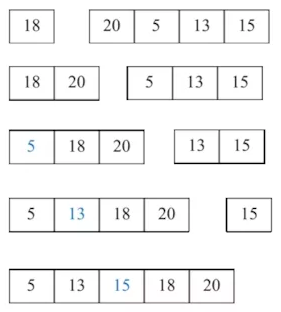
\includegraphics[scale=0.7]{ins_sort.png}}
	\caption{Сортировка вставками.}
	\label{fig:ins_s}
\end{figure}

\newpage

\section{Быстрая сортировка}
Общая идея алгоритма состоит в следующем:

\begin{itemize}
	\item выбрать из массива элемент, называемый опорным. Это может быть любой из элементов массива. От выбора опорного элемента не зависит корректность алгоритма, но в отдельных случаях может сильно зависеть его эффективность 
	\item сравнить все остальные элементы с опорным и переставить их в массиве так, чтобы разбить массив на три непрерывных отрезка, следующих друг за другом: «элементы меньшие опорного», «равные» и «большие».
	\item для отрезков «меньших» и «больших» значений выполнить рекурсивно ту же последовательность операций, если длина отрезка больше единицы.
\end{itemize}

На практике массив обычно делят не на три, а на две части: например, «меньшие опорного» и «равные и большие»; такой подход в общем случае эффективнее, так как упрощает алгоритм разделения.

\section{Вывод}
	В данном разделе были рассмотрены 3 алгоритмы сортировки: пузырьком, вставками и быстрая сортировка.
	
\clearpage

\chapter{Конструкторская часть}

\section{Схемы алгоритмов}
В данной части будут рассмотрены схемы алгоритмов сортировки пузырьком, вставками и быстрой сортировки. На рисунках 2.1 - 2.3 представлены рассматриваемые алгоритмы.

\begin{figure}[h]
	\centering
	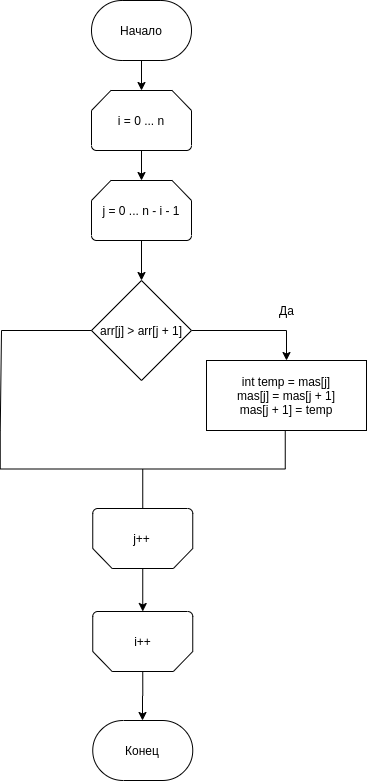
\includegraphics[width=0.4\linewidth]{bsort.jpg}
	\caption{Схема сортировки пузырьком}
	\label{fig:mpr}
\end{figure}

\newpage

\begin{figure}[h]
	\centering
	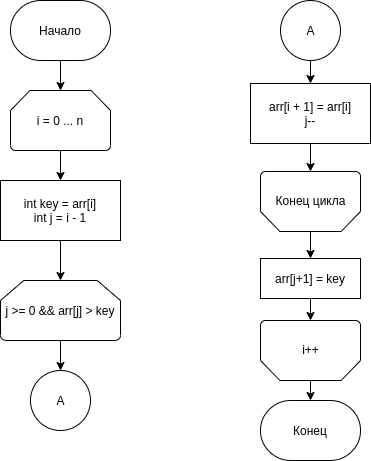
\includegraphics[scale=1]{isort.jpg}
	\caption{Схема сортировки вставками}
	\label{fig:mpr}
\end{figure}

\newpage

\begin{figure}[h]
	\centering
	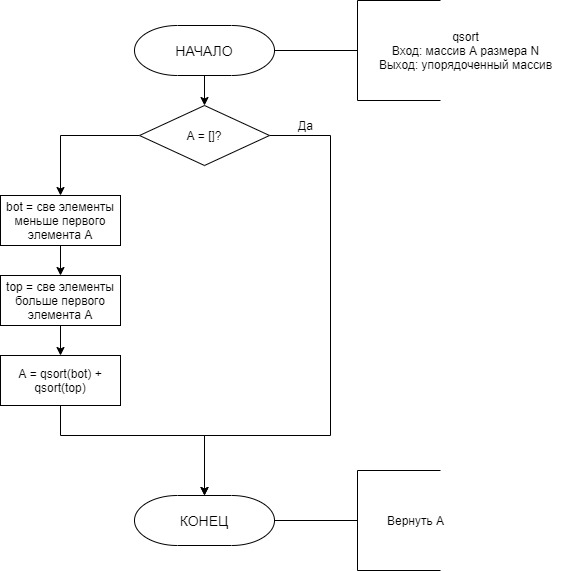
\includegraphics[scale=0.8]{qsort.jpg}
	\caption{Схема быстрой сортировк}
	\label{fig:mpr}
\end{figure}

\newpage

\section{Модель вычислений}

Для последующего вычисления трудоемкости введём модель вычислений:

\begin{enumerate}
	\item Операции из списка (\ref{for:opers}) имеют трудоемкость 1.
	\begin{equation}
		\label{for:opers}
		+, -, /, \%, ==, !=, <, >, <=, >=, [], ++, {-}-
	\end{equation}
	\item Трудоемкость оператора выбора if условие then A else B рассчитывается, как (\ref{for:if}).
	\begin{equation}
		\label{for:if}
		f_{if} = f_{\text{условия}} +
		\begin{cases}
			f_A, & \text{если условие выполняется,}\\
			f_B, & \text{иначе.}
		\end{cases}
	\end{equation}
	\item Трудоемкость цикла рассчитывается, как (\ref{for:for}).
	\begin{equation}
		\label{for:for}
		f_{for} = f_{\text{инициализации}} + f_{\text{сравнения}} + N(f_{\text{тела}} + f_{\text{инкремента}} + f_{\text{сравнения}})
	\end{equation}
	\item Трудоемкость вызова функции равна 0.
\end{enumerate}

\section{Трудоёмкость алгоритмов}

Пусть размер массивов во всех вычислениях обозначается как $N$.

\subsection{Алгоритм сортировки пузырьком}

Трудоёмкость алгоритма сортировки пузырьком состоит из:
\begin{itemize}
	\item трудоёмкость сравнения и инкремента внешнего цикла $i \in [1..N)$ (\ref{for:bubble_outer}):
	\begin{equation}
		\label{for:bubble_outer}
		f_{i} = 2 + 2(N - 1)
	\end{equation}
	\item суммарная трудоёмкость внутренних циклов, количество итераций которых меняется в промежутке $[1..N-1]$ (\ref{for:bubble_inner}):
	\begin{equation}
		\label{for:bubble_inner}
		f_{j} = 3(N - 1) + \frac{N \cdot (N - 1)}{2} \cdot (3 + f_{if})
	\end{equation}
	\item трудоёмкость условия во внутреннем цикле (\ref{for:bubble_if}):
	\begin{equation}
		\label{for:bubble_if}
		f_{if} = 4 + \begin{cases}
			0, & \text{в лучшем случае}\\
			9, & \text{в худшем случае}\\
		\end{cases}
	\end{equation}
\end{itemize}

Трудоёмкость в \textbf{лучшем} случае (\ref{for:bubble_best}):
\begin{equation}
	\label{for:bubble_best}
	f_{best} = \frac{7}{2} N^2 + \frac{3}{2} N - 3 \approx \frac{7}{2} N^2 = O(N^2)
\end{equation}

Трудоёмкость в \textbf{худшем} случае (\ref{for:bubble_worst}):
\begin{equation}
	\label{for:bubble_worst}
	f_{worst} =  8N^2 - 8N - 3 \approx 8N^2 = O(N^2)
\end{equation}

\subsection{Алгоритм сортировки вставками}

Трудоёмкость алгоритма сортировки пузырьком состоит из:
\begin{itemize}
	\item трудоёмкость сравнения и инкремента внешнего цикла $i \in [1..N)$ (\ref{for:isort_outer}):
	\begin{equation}
		\label{for:isort_outer}
		f_{i} = 2 + 2(N - 1)
	\end{equation}
	\item суммарная трудоёмкость внутренних циклов, количество итераций которых меняется в промежутке $[1..N-1]$ (\ref{for:isort_inner}):
	
	\begin{equation}
		\label{for:isort_inner}
		f_{if} = 4 + \begin{cases}
			0, & \text{в лучшем случае}\\
			3(N - 1) + \frac{N \cdot (N - 1)}{2} \cdot (3 + f_{if}), & \text{в худшем случае}\\
		\end{cases}
	\end{equation}
	
	\item трудоёмкость условия во внутреннем цикле (\ref{for:isort_if}):
	\begin{equation}
		\label{for:isort_if}
		f_{if} = 4 + \begin{cases}
			0, & \text{в лучшем случае}\\
			9, & \text{в худшем случае}\\
		\end{cases}
	\end{equation}
\end{itemize}

Трудоёмкость в \textbf{лучшем} случае (\ref{for:isort_best}):
\begin{equation}
	\label{for:isort_best}
	f_{best} = 13N - 10 \approx 13N = O(N)
\end{equation}

Трудоёмкость в \textbf{худшем} случае (\ref{for:isort_worst}):
\begin{equation}
	\label{for:isort_worst}
	f_{worst} = 4.5N^2 + 10N - 13 \approx 4N^2 = O(N^{2})
\end{equation}

\section{Вывод}
	На основе теоретических данных, полученных из аналитического раздела, были построены схемы трёх алгоритмов сортировки. Оценены их тредёмкости в лучшем и худшем случаях.

\chapter{Технологическая часть}

\section{Выбор ЯП}
В данной лабораторной работе использовался язык программирования - python. Данный выбор обусловлен тем, что этот язык наиболее удобен для работы со строками, а также тем, что в нём присутсвует функция для измерения процессорного времени.
В качестве среды разработки я использовала Visual Studio Code, так как считаю его достаточно удобным.

\section{Требование к ПО}
К программе предъявляется ряд требований:

\begin{itemize}
	\item на вход ПО получает массив сравнимых элементов;
	\item на выходе -- тот же массив, но отсортированный в заданном порядке.
\end{itemize}

\section{Реализация алгоритмов}

В листингах 3.1 - 3.3 приведена реализация трёх алгоритмов сортировки.

\begin{lstlisting}[label=some-code,caption=Функция сортировки массива пузырьком,language=Python]
def bubble(arr):
	for i in range(len(arr)):
		for j in range(len(arr)-i-1):
			if arr[j] > arr[j+1]:
				arr[j], arr[j+1] = arr[j+1], arr[j]
	return arr
\end{lstlisting}

\begin{lstlisting}[label=some-code,caption=Функция сортировки массива вставками,language=Python]
def insertion(arr):
	for i in range(len(arr)):
		current = arr[i]
		j = i
		while (arr[j-1] > current) and (j > 0):
			arr[j] = arr[j-1]
			j = j - 1
		arr[j] = current
	return arr
\end{lstlisting}

\begin{lstlisting}[label=some-code,caption=Функция быстрой сортировки,language=Python]
def quick(arr):
	if len(arr) <= 1:
		return arr
	else:
		q = arr[0]
		s_nums = []
		m_nums = []
		e_nums = []
		for n in arr:
			if n < q:
				s_nums.append(n)
			elif n > q:
				m_nums.append(n)
			else:
				e_nums.append(n)
		return quick(s_nums) + e_nums + quick(m_nums)
\end{lstlisting}

\section{Тестовые данные}

В таблице~\ref{tbl:test} приведены тесты для функций, реализующих алгоритмы сортировки. Все тесты пройдены успешно.

\begin{table}[h!]
	\begin{center}
		\caption{\label{tbl:test}Тестирование функций}
		\begin{tabular}{|c|c|c|}
			\hline
			Входной массив & Результат & Ожидаемый результат \\ 
			\hline
			$[8, 12, 17, 25, 34]$ & $[8, 12, 17, 25, 34]$  & $[8, 12, 17, 25, 34]$\\\hline
			$[41, 35, 21, 17, 5]$  & $[5, 17, 21, 35, 41]$ & $[5, 17, 21, 35, 41]$\\\hline
			$[-7, -12, -32, -78, -92]$  & $[-92, -78, -32, -12, -7]$  & $[-92, -78, -32, -12, -7]$\\\hline
			$[35, -7, 12, -51, 101]$  & $[-51, -7, 12, 35, 51]$  & $[-51, -7, 12, 35, 51]$\\\hline
			$[10]$  & $[10]$  & $[10]$\\\hline
			$[-3]$  & $[-3]$  & $[-3]$\\\hline
			Пустой массив  & Пустой массив  & Пустой массив\\
			\hline
		\end{tabular}
	\end{center}
\end{table}

\section{Вывод}
В данном разделе были разработаны исходные коды трёх алгоритмов сортировки: пузырьком, вставками и быстрая сортировка..

\chapter{Исследовательская часть}

\section{Пример работы}

Демонстрация работы программы приведена на рисунке 4.1.

\begin{figure}[h]
	\begin{center}
	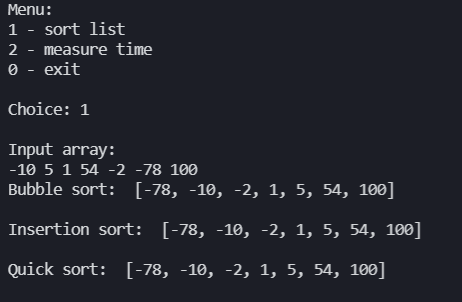
\includegraphics[scale=1.3]{example.png}
	 \caption{Работа алгоритмов сортировки}
	\end{center}
\end{figure}

\section{Время выполнения алгоритмов}
Время выполнения алгоритмов замерялось с помощью функции process\_time модуля time в Python.

\begin{table} [h!]
	\caption{Таблица времени выполнения сортировок на случайных данных}
	\begin{center}
		\begin{tabular}{|c c c c|}
			
			\hline
			
			Размер & bsort & isort  & qsort \\ [0.5ex]
			
			1000 & 0.453125 & 0.281250 & 0.015625 \\ 
			
			\hline 
			
			2000 & 1.796875 & 1.125000 & 0.046875 \\ 
			
			\hline 
			
			3000 & 4.046875 & 2.421875 & 0.093750 \\ 
			
			\hline 
			
			5000 & 11.296875 & 7.015625 & 0.140625 \\ 
			
			\hline 
			
		\end{tabular}
	\end{center}
\end{table}

\newpage

\begin{figure}[h!]
	\begin{center}
		\begin{tikzpicture}
			\begin{axis}[
				legend pos = north west,
				xlabel=размер,
				ylabel=секунды,
				minor tick num = 1,
				grid = both,
				major grid style = {lightgray},
				minor grid style = {lightgray!25},
				xtick distance = 1000,
				width = 0.9\textwidth,
				height = 0.5\textwidth]
				
				\addplot[
				blue,
				semithick,
				mark = x,
				mark size = 3pt,
				thick,
				] file {bsort.txt};
				
				\addplot[
				red,
				semithick,
				mark = x,
				mark size = 3pt,
				thick,
				] file {isort.txt};
				
				\addplot[
				green,
				semithick,
				mark = x,
				mark size = 3pt,
				thick,
				] file {qsort.txt};
				
				\legend{
					сортировка пузырьком,
					сортировка вставками,
					быстрая сортировка
				}
			\end{axis}
		\end{tikzpicture}
	\end{center}
	\caption{Сравнение времени выполнения сортировок на случайных данных}
\end{figure}

\section{Вывод}

При прямом порядке элементов в массиве, сортировка пузьком работает медленее чем сортировка вставками, и ещё медленее чем быстрая.


\chapter*{Заключение}
\addcontentsline{toc}{chapter}{Заключение}

На основании анализа трудоемкости алгоритмов в выбранной модели вычислений, было показано, что алгоритм сортировки вставками имеет наименьшую сложность (линейную) в уже отсортированном массиве. В случае обранто отсортированного массива, сортировка вставками и пузырьком имееют квадратическую сложность. На основании замеров времени исполнения алгоритмов, был сделан вывод, что при прямом порядке элементов в массиве, сортировка пузьком работает медленее чем быстрая и еще медленее чем сортировка вставкам. Так же был доказана выведенная трудоемкость алгоритма сортировки вставками -- при  уже отсортированном массиве сортировка работает очень быстро. На случайных данных быстрее всех работает алгоритм быстрой сортировки.

\addcontentsline{toc}{chapter}{Список литератури}

\bibliographystyle{utf8gost705u}  % стилевой файл для оформления по ГОСТу

\bibliography{51-biblio}          % имя библиографической базы (bib-файла)

\begin{thebibliography}{9}
	\bibitem{Academy} Основные виды сортировок и примеры их реализации. [Электронный ресурс]. Режим доступа: 
	
	https://academy.yandex.ru/posts/osnovnye-vidy-sortirovok-i-primery-ikh-realizatsii
	{Дата обращения: 17.10.2021}
	
	\bibitem{habr} Описание алгоритмов сортировки и сравнение их производительности. [Электронный ресурс.] Режим доступа:
	
	https://habr.com/ru/post/335920/
	{Дата обращения: 17.10.2021}
	
	\bibitem{habr_alg} Знай сложности алгоримтмов. [Электронный ресурс.] Режим доступа:
	
	https://habr.com/ru/post/188010/
	{Дата обращения: 17.10.2021}
	
	\bibitem{python} Python documentation. [Электронный ресурс.] Режим доступа:
	
	https://www.python.org/doc/
	{Дата обращения: 17.10.2021}
\end{thebibliography}

\end{document}
